\documentclass[12pt,a4paper]{report}
\special{papersize=210mm,297mm}

\usepackage{amsmath}			%
\usepackage{blindtext}			%
\usepackage{booktabs}           % For prettier tables
\usepackage{enumitem}			%
\usepackage{gensymb}			%
\usepackage{geometry}			%
\usepackage{graphicx}			%
\usepackage{hyperref}			%
\usepackage[utf8]{inputenc}		%
\usepackage[english]{isodate}	%
\usepackage{longtable}			%
\usepackage{setspace}			%
\usepackage{siunitx}			% Required for alignment

\frenchspacing

%\linespread{1.3}
%\onehalfspacing
\setstretch{1.3}

\setlength{\parindent}{1em}
\setlength{\parskip}{1em}

\tolerance=1000
\hyphenpenalty=100000

\isodate

\title{Flight Dynamics Model for the Real-Time Flight Simulation}
\author{Marek Cel}
\date{}

\begin{document}
  
  \begin{titlepage}
    \centering
    {\huge Flight Dynamics Model for the Real-Time Flight Simulation\par}
  \end{titlepage}
  
  %\maketitle

  \noindent Copyright \copyright{} \the\year{} Marek M. Cel. All rights reserved.

  \noindent Author: Marek M. Cel \\
  Revision: 10 \\
  Date: \today

  \noindent This work is licensed under a \newline
\textbf{Creative Commons CC0 1.0 Universal Public Domain Dedication}

\noindent \textbf{Statement of Purpose}

\noindent The laws of most jurisdictions throughout the world
automatically confer exclusive Copyright and Related Rights
(defined below) upon the creator and subsequent owner(s) (each
and all, an ``owner'') of an original work of authorship and/or
a database (each, a ``Work'').

\noindent Certain owners wish to permanently relinquish those rights
to a Work for the purpose of contributing to a commons of
creative, cultural and scientific works (``Commons'') that the
public can reliably and without fear of later claims of
infringement build upon, modify, incorporate in other works,
reuse and redistribute as freely as possible in any form
whatsoever and for any purposes, including without limitation
commercial purposes. These owners may contribute to the
Commons to promote the ideal of a free culture and the further
production of creative, cultural and scientific works, or to
gain reputation or greater distribution for their Work in part
through the use and efforts of others.

\noindent For these and/or other purposes and motivations, and
without any expectation of additional consideration or
compensation, the person associating CC0 with a Work (the
``Affirmer''), to the extent that he or she is an owner of
Copyright and Related Rights in the Work, voluntarily elects
to apply CC0 to the Work and publicly distribute the Work
under its terms, with knowledge of his or her Copyright and
Related Rights in the Work and the meaning and intended legal
effect of CC0 on those rights.

\noindent \textbf{1. Copyright and Related Rights.}
A Work made available under CC0 may be protected by
copyright and related or neighboring rights (``Copyright and
Related Rights''). Copyright and Related Rights include, but
are not limited to, the following:

\begin{enumerate}[noitemsep,label=\roman*.]
  
  \item the right to reproduce, adapt, distribute, perform,
  display, communicate, and translate a Work;
  
  \item  moral rights retained by the original author(s) and/or
  performer(s);
  
  \item publicity and privacy rights pertaining to a person's
  image or likeness depicted in a Work;
  
  \item rights protecting against unfair competition in regards
  to a Work, subject to the limitations in paragraph 4(a),
  below;
  
  \item rights protecting the extraction, dissemination, use and
  reuse of data in a Work;
  
  \item database rights (such as those arising under Directive
  96/9/EC of the European Parliament and of the Council of 11
  March 1996 on the legal protection of databases, and under
  any national implementation thereof, including any amended
  or successor version of such directive); and
  
  \item other similar, equivalent or corresponding rights
  throughout the world based on applicable law or treaty, and
  any national implementations thereof.

\end{enumerate}

\noindent \textbf{2. Waiver.} To the greatest extent
permitted by, but not in contravention of, applicable law,
Affirmer hereby overtly, fully, permanently, irrevocably and
unconditionally waives, abandons, and surrenders all of
Affirmer's Copyright and Related Rights and associated claims
and causes of action, whether now known or unknown (including
existing as well as future claims and causes of action), in
the Work (i) in all territories worldwide, (ii) for the
maximum duration provided by applicable law or treaty
(including future time extensions), (iii) in any current or
future medium and for any number of copies, and (iv) for any
purpose whatsoever, including without limitation commercial,
advertising or promotional purposes (the ``Waiver''). Affirmer
makes the Waiver for the benefit of each member of the public
at large and to the detriment of Affirmer's heirs and
successors, fully intending that such Waiver shall not be
subject to revocation, rescission, cancellation, termination,
or any other legal or equitable action to disrupt the quiet
enjoyment of the Work by the public as contemplated by
Affirmer's express Statement of Purpose.

\noindent \textbf{3. Public License Fallback.} Should any
part of the Waiver for any reason be judged legally invalid or
ineffective under applicable law, then the Waiver shall be
preserved to the maximum extent permitted taking into account
Affirmer's express Statement of Purpose. In addition, to the
extent the Waiver is so judged Affirmer hereby grants to each
affected person a royalty-free, non transferable, non
sublicensable, non exclusive, irrevocable and unconditional
license to exercise Affirmer's Copyright and Related Rights
in the Work (i) in all territories worldwide, (ii) for the
maximum duration provided by applicable law or treaty
(including future time extensions), (iii) in any current or
future medium and for any number of copies, and (iv) for any
purpose whatsoever, including without limitation commercial,
advertising or promotional purposes (the ``License''). The
License shall be deemed effective as of the date CC0 was
applied by Affirmer to the Work. Should any part of the
License for any reason be judged legally invalid or
ineffective under applicable law, such partial invalidity or
ineffectiveness shall not invalidate the remainder of the
License, and in such case Affirmer hereby affirms that he or
she will not (i) exercise any of his or her remaining
Copyright and Related Rights in the Work or (ii) assert any
associated claims and causes of action with respect to the
Work, in either case contrary to Affirmer's express Statement
of Purpose.

\noindent \textbf{4. Limitations and Disclaimers.}

\begin{enumerate}[noitemsep,label=\alph*.]
  
  \item No trademark or patent rights held by Affirmer are
  waived, abandoned, surrendered, licensed or otherwise
  affected by this document.
  
  \item Affirmer offers the Work as-is and makes no
  representations or warranties of any kind concerning the
  Work, express, implied, statutory or otherwise, including
  without limitation warranties of title, merchantability,
  fitness for a particular purpose, non infringement, or the
  absence of latent or other defects, accuracy, or the present
  or absence of errors, whether or not discoverable, all to
  the greatest extent permissible under applicable law.
  
  \item Affirmer disclaims responsibility for clearing rights of
  other persons that may apply to the Work or any use thereof,
  including without limitation any person's Copyright and
  Related Rights in the Work. Further, Affirmer disclaims
  responsibility for obtaining any necessary consents,
  permissions or other rights required for any use of the
  Work.
  
  \item Affirmer understands and acknowledges that Creative
  Commons is not a party to this document and has no duty or
  obligation with respect to this CC0 or use of the Work.

\end{enumerate}

  
  {
    \clearpage
    \setlength{\parskip}{0em}
    \pdfbookmark{\contentsname}{toc}
    \tableofcontents
  }

  \clearpage %or \cleardoublepage
\phantomsection
\chapter*{Notation}
\markright{}
\addcontentsline{toc}{chapter}{Notation}

\begin{longtable}[l]{ l l p{0.6\textwidth} }
  $a$                                                    & -- & [m] ellipsoid equatorial radius \\
  $a=\frac{dC_L}{da}$                                    & -- & [1/rad] lift curve slope \\
  $A_R=\pi R^2$                                          & -- & [m\textsuperscript{2}] rotor disc area \\
  $b$                                                    & -- & [m] ellipsoid polar radius \\
  $b$                                                    & -- & [m] wing span \\
  $B$                                                    & -- & [-] blade tip loss factor \\
  $c$                                                    & -- & [m] mean aerodynamic chord \\
  $c$                                                    & -- & [N/(m/s)] damping coefficient \\
  $c_B$                                                  & -- & [m] rotor blade chord \\
  $c_S$                                                  & -- & [m/s] speed of sound \\
  $C_D$                                                  & -- & [-] drag coefficient \\
  $C_l$                                                  & -- & [-] rolling moment coefficient \\
  $C_L$                                                  & -- & [-] lift coefficient \\
  $C_m$                                                  & -- & [-] pitching moment coefficient \\
  $C_n$                                                  & -- & [-] yawing moment coefficient \\
  $C_P$                                                  & -- & [-] power coefficient \\
  $C_T$                                                  & -- & [-] thrust coefficient \\
  $C_Y$                                                  & -- & [-] side force coefficient \\
  $C_{\Delta P}$                                         & -- & [-] engine power losses coefficient \\
  $D$                                                    & -- & [N] drag \\
  $D$                                                    & -- & [m] propeller diameter \\
  $e$                                                    & -- & [m] flapping hinge offset \\
  $g$                                                    & -- & [m/s\textsuperscript{2}] gravitational acceleration \\
  $h$                                                    & -- & [m] altitude \\
  $\vec H=\left[ H_X, H_Y, H_Z \right]^T$                & -- & [kg$\cdot$m\textsuperscript{2}/s] angular momentum vector \\
  $i$                                                    & -- & [rad] incidence angle \\
  $I_B$                                                  & -- & [kg$\cdot$m\textsuperscript{2}] rotor blade moment of inertia \\
  $\boldsymbol I$                                        & -- & [kg$\cdot$m\textsuperscript{2}] inertia matrix \\
  $J$                                                    & -- & [-] propeller advance ratio \\
  $k$                                                    & -- & [N/m] spring constant \\
  $L$                                                    & -- & [N] lift \\
  $L$                                                    & -- & [m] reference length scale \\
  $m$                                                    & -- & [kg] mass \\
  $\boldsymbol M$                                        & -- & [kg],[kg$\cdot$m],[kg$\cdot$m\textsuperscript{2}] generalized inertia matrix \\
  $n$                                                    & -- & [rpm] engine revolutions per minute \\
  $n$                                                    & -- & [rev./s] propeller revolution speed \\
  $N_B$                                                  & -- & number of rotor blades \\
  $p$                                                    & -- & [Pa] pressure \\
  $P$                                                    & -- & [W] power \\
  $\vec P=\left[ P_X, P_Y, P_Z \right]^T$                & -- & [kg$\cdot$m/s] momentum vector \\
  $Q$                                                    & -- & [N$\cdot$m] torque \\
  $\vec Q=\left[ L, M, N \right]^T$                      & -- & [N$\cdot$m] moment of force vector \\
  $r$                                                    & -- & [m] coordinate along blade span \\
  $\vec r=\left[ x, y, z \right]^T$                      & -- & [m] coordinates vector \\
  $R$                                                    & -- & [N$\cdot$m/(kmol$\cdot$K)] universal gas constant \\
  $R$                                                    & -- & [m] rotor radius \\
  $\vec R=\left[ X, Y, Z \right]^T$                      & -- & [N] force vector \\
  $Re$                                                   & -- & [-] Reynolds number \\
  $s=\frac{N_B c_B}{\pi R}$                              & -- & [-] rotor solidity \\
  $\boldsymbol s=\left[ u,v,w,p,q,r \right]^T$           & -- & [m/s],[rad/s] aircraft state vector \\
  $S$                                                    & -- & [m\textsuperscript{2}] wing area \\
  $S$                                                    & -- & [K] Sutherland constant \\
  $S_B$                                                  & -- & [kg$\cdot$m] blade first moment of mass \\
  $\vec S=\left[ S_X, S_Y, S_Z \right]^T$                & -- & [kg$\cdot$m] first moment of mass \\
  $T$                                                    & -- & [K] temperature \\
  $T$                                                    & -- & [N] thrust \\
  $V$                                                    & -- & [m/s] velocity \\
  $V_I$                                                  & -- & [m/s] induced velocity \\
  $V_IH$                                                 & -- & [m/s] induced velocity for hovering \\
  $\vec V=\left[ u, v, w \right]^T$                      & -- & [m/s] velocity vector \\
  $\boldsymbol x=\left[ x,y,z,e_0,e_x,e_y,e_z \right]^T$ & -- & [m],[-] aircraft coordinates vector \\
  $\alpha$                                               & -- & [rad] angle of attack \\
  $\beta$                                                & -- & [rad] angle of sideslip \\
  $\beta$                                                & -- & [rad] rotor blade flapping angle \\
  $\beta_0$                                              & -- & [rad] rotor coning angle \\
  $\beta_1c$, $\beta_1s$                                 & -- & [rad] longitudinal and lateral tip-path angles \\
  $\gamma=\frac{\rho a c_B R^2}{I_B}$                    & -- & [-] blade Lock number \\
  $\hat \delta$                                          & -- & [-] normalized controls position \\
  $\varepsilon$                                          & -- & [rad] rotor shaft inclination angle \\
  $\theta_0$                                             & -- & [rad] collective pitch angle \\
  $\theta_1s$, $\theta_1c$                               & -- & [rad] longitudinal and lateral cyclic pitch angle \\
  $\Theta$                                               & -- & [rad] pitch angle \\
  $\lambda$                                              & -- & [rad] geographic longitude \\
  $\lambda=\frac{w_{rw} - V_I}{\Omega_R R}$              & -- & [-] rotor inflow ratio \\
  $\lambda_I=\frac{V_I}{\Omega_R R}$                     & -- & [-] induced inflow ratio \\
  $\lambda_IH=\frac{V_IH}{\Omega_R R}$                   & -- & [-] induced inflow ratio for hovering \\
  $\mu$                                                  & -- & [-] friction coefficient \\
  $\mu$                                                  & -- & [Pa$\cdot$s] dynamic viscosity \\
  $\mu=\frac{V}{\Omega_R R}$                             & -- & [-] rotor advance ratio \\
  $\mu_C=\frac{V_C}{\Omega_R R}$                         & -- & [-] normalized climb velocity \\
  $\mu_D=\frac{V_D}{\Omega_R R}$                         & -- & [-] normalized descent velocity \\
  $\nu$                                                  & -- & [m\textsuperscript{2}/s] kinematic viscosity \\
  $\rho$                                                 & -- & [kg/m\textsuperscript{3}] air density \\
  $\varphi$                                              & -- & [rad] geographic latitude \\
  $\Phi$                                                 & -- & [rad] roll angle \\
  $\chi$                                                 & -- & [rad] rotor wake angle \\
  $\Psi$                                                 & -- & [rad] yaw angle \\
  $\Psi$                                                 & -- & [rad] rotor blade azimuth \\
  $\vec \Omega=\left[ p, q, r \right]^T$                 & -- & [rad/s] angular velocity vector \\
  $\Omega_R$                                             & -- & [rad/s] rotor revolution speed \\
  $\frac{\epsilon}{\alpha}$                              & -- & [-] horizontal stabilizer downwash angle derivative with respect to the aircraft angle of attack \\
\end{longtable}

\noindent \textbf{Indices:}

\begin{longtable}[l]{ l l l }
  $AC$  & -- & aerodynamic center \\
  $a$   & -- & Aerodynamic Axis System \\
  $b$   & -- & Body Axis System \\
  $ba$  & -- & Blade Axis System \\
  $B$   & -- & rotor blade \\
  $c$   & -- & Control Axis System \\
  $cw$  & -- & Control-Wind Axis System \\
  $C$   & -- & climb \\
  $CM$  & -- & Center of Mass \\
  $D$   & -- & descent \\
  $g$   & -- & Gravity (North-East-Down) Axis System \\
  $h$   & -- & horizontal stabilizer \\
  $I$   & -- & induced \\
  $IH$  & -- & induced in hovering \\
  $MAP$ & -- & manifold absolute pressure \\
  $N$   & -- & normal \\
  $O$   & -- & coordinate system’s origin \\
  $r$   & -- & Rotor Axis System \\
  $rw$  & -- & Rotor-Wind Axis System \\
  $R$   & -- & rotor \\
  $RH$  & -- & rotor hub \\
  $s$   & -- & Stability Axis System \\
  $T$   & -- & tangent \\
  $v$   & -- & vertical stabilizer \\
  $X$   & -- & x-axis component \\
  $Y$   & -- & y-axis component \\
  $Z$   & -- & z-axis component \\
\end{longtable}

\noindent \textbf{Derivatives:}

\begin{longtable}[l]{ l l l }
  $\dot u=\frac{du}{dt}$             & -- & time derivative \\
  $\bar \beta=\frac{d\beta}{d\Psi}$  & -- & azimuth derivative \\
\end{longtable}

  \chapter{Introduction}

% This document describes fligh dynamics model used by the MScSim flight simulation software.

\section{Conventions}

Flight Dynamics Model uses International System of Units (SI) for all internal computations. It is clearly specified if other units are used.

All rotations and rotation related operations are considered to be a passive (alias) rotations.

\section{Coordinates Systems}

\subsection{Body Axis System}

Body Axis System is body-centered, body-fixed coordinate system, with the x\nobreakdash-axis positive forwards, the y\nobreakdash-axis positive right and the z\nobreakdash-axis positive downwards.

\begin{figure}
  \centering
  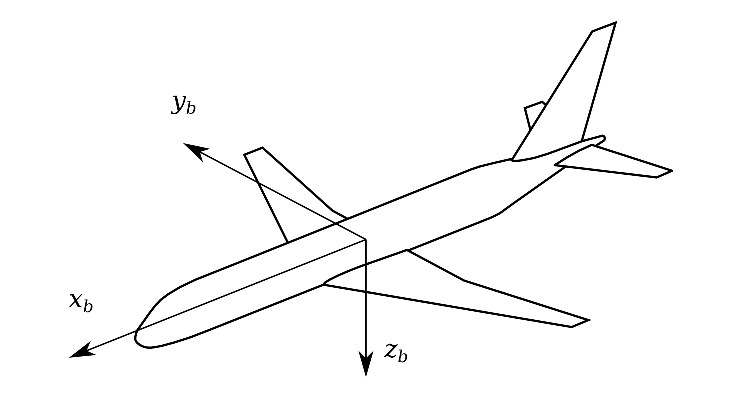
\includegraphics[width=110mm]{images/coordinate_system_BAS.eps}
  \caption{Body Axis System}
\end{figure}

\subsection{Stability Axis System}

Origin of the Stability Axis System is coincident with the origin of the Body Axis System, the x\nobreakdash-axis is directed along air freestream velocity vector projected onto the XZ plane of the Body Axis System, the y\nobreakdash-axis is coincident with the the y\nobreakdash-axis of the Body Axis System, and the z\nobreakdash-axis completes a right-handed coordinate system.

\begin{figure}
  \centering
  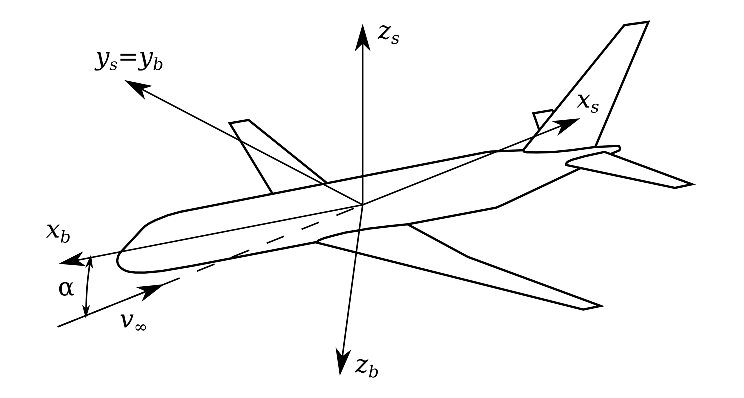
\includegraphics[width=110mm]{images/coordinate_system_Stab.eps}
  \caption{Stability Axis System}
\end{figure}

\subsection{Aerodynamic Axis System}

Origin of the Aerodynamic Axis System is coincident with the origin of the Body Axis System, the x\nobreakdash-axis is directed along air freestream velocity vector, the z\nobreakdash-axis lies in the aircraft plane of symmetry pointing upwards, and the y\nobreakdash-axis completes a right-handed coordinate system.

\begin{figure}
  \centering
  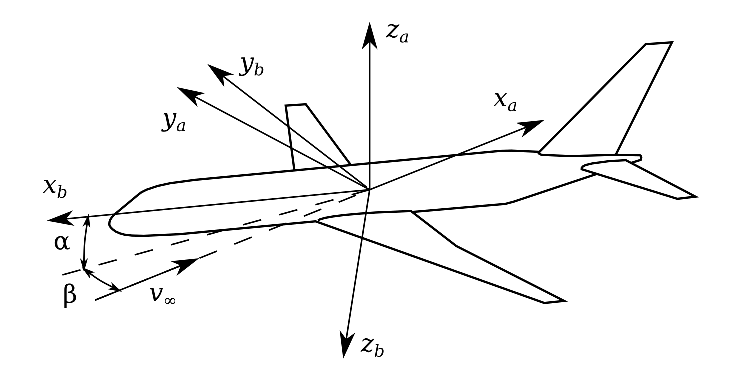
\includegraphics[width=110mm]{images/coordinate_system_Aero.eps}
  \caption{Aerodynamic Axis System}
\end{figure}

\subsection{Gravity Axis System}

There are basically two conventions of Gravity Axis Systems used for the purpose of flight dynamics East\nobreakdash-North\nobreakdash-Up and North\nobreakdash-East\nobreakdash-Down.

It is convenient to use North-East-Down axes system together with the Body Axis System and Bryant angles (Euler angles in z\nobreakdash-y\nobreakdash-x convention) as those angles in NED frame become aircraft heading, pitch and roll.

Considering all this, Gravity Earth Axis System is a coordinate system, with the x\nobreakdash-axis positive North, the y\nobreakdash-axis positive East and z\nobreakdash-axis positive downwards.

\subsection{Earth-fixed Axis System}

For any further considerations World Geodetic System 1984 as described in \cite{NIMA-TR-8350-2} is used as the Earth-fixed Axis System.

\begin{figure}
  \centering
  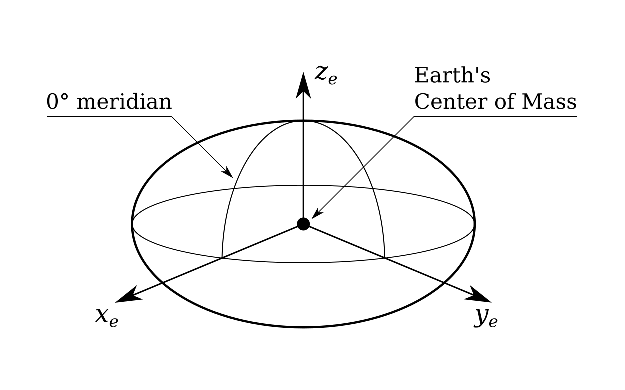
\includegraphics[width=90mm]{images/coordinate_system_WGS.eps}
  \caption{World Geodetic System 1984}
\end{figure}

\section{Aircraft Attitude}

\begin{figure}[h!]
  \centering
  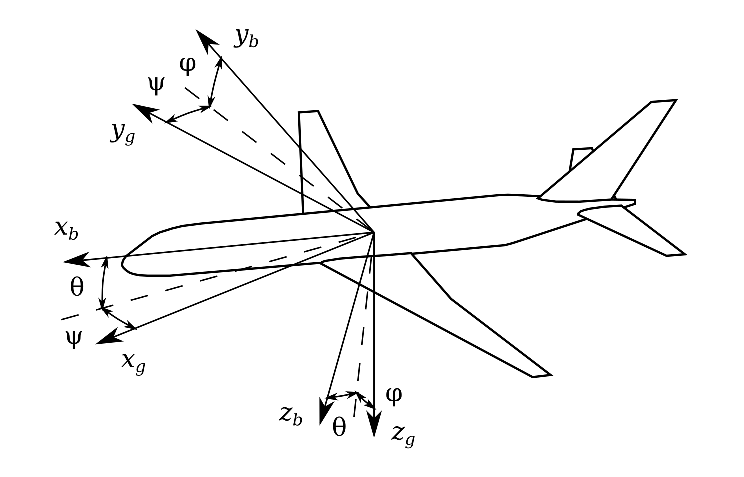
\includegraphics[width=110mm]{images/roll_pitch_yaw.eps}
  \caption{Tait–Bryan angles}
\end{figure}

Aircraft attitude is defined either by a quaternion or by quasi-Euler Tait-Bryan $\psi$\nobreakdash-$\theta$\nobreakdash-$\phi$ angles in z\nobreakdash-y\nobreakdash-x convention. It is convenient to use such a convention, as this angles becomes aircraft roll, pitch and heading when expressed in North\nobreakdash-East\nobreakdash-Down coordinate system.

\section{Transformations Between Coordinates Systems}

\subsection{Rotation Matrices}

ransformation to the coordinate system rotated by Tait-Bryan $\psi$\nobreakdash-$\theta$\nobreakdash-$\phi$ angles can be performed using rotation matrix, which is given by the following relations. \cite{Padfield2007, Sibilski2004}
\begin{align}
  \boldsymbol T \left( \phi \right) &=
  \left[
    \begin{matrix}
      1 &          0 &         0 \\
      0 &  \cos \phi & \sin \phi \\
      0 & -\sin \phi & \cos \phi \\
    \end{matrix}
  \right]
  \\
  \boldsymbol T \left( \theta \right) &=
  \left[
    \begin{matrix}
      \cos \theta & 0 & -\sin \theta \\
                0 & 1 &            0 \\
      \sin \theta & 0 &  \cos \theta \\
    \end{matrix}
  \right]
  \\
  \boldsymbol T \left( \psi \right) &=
  \left[
    \begin{matrix}
       \cos\psi & \sin\psi & 0 \\
      -\sin\psi & \cos\psi & 0 \\
              0 &        0 & 1 \\
    \end{matrix}
  \right]
\end{align}

\begin{equation}
  \begin{array}{c}
  \boldsymbol T \left( \phi,\theta,\psi \right) =
  \boldsymbol T \left( \phi \right)
  \boldsymbol T \left( \theta \right) 
  \boldsymbol T \left( \psi \right) = \\
  \left[
    \begin{matrix}
       \cos \theta \cos \psi &
       \cos \theta \sin \psi &
      -\sin \theta \\
       \cos \psi   \sin \phi   \sin \theta - \cos \phi   \sin \psi &
       \cos \phi   \cos \psi + \sin \phi     \sin \theta \sin \psi &
       \cos \theta \sin \phi \\
       \sin \phi   \sin \psi + \cos \phi     \cos \psi   \sin \theta &
       \cos \phi   \sin \theta \sin \psi   - \cos \psi   \sin \phi &
       \cos \phi   \cos \theta \\
    \end{matrix}
  \right]
  \end{array}
\end{equation}

\subsection{Geographic Coordinates}

\subsubsection{Conversion from Geographic to Cartesian Coordinates}

Procedure of conversion from geographic coordinates to the Cartesian coordinates system is given as follows.
\begin{align}
  e    &= \frac{1}{a} \sqrt{a^2-b^2} \\
  \chi &= \sqrt{ 1 - e^2 \sin^2 \varphi } \\
  x_e  &= \left( \frac{a}{\chi} + h \right) \cos \varphi \cos \lambda \\
  y_e  &= \left( \frac{a}{\chi} + h \right) \cos \varphi \sin \lambda \\
  z_e  &= \left( a \frac{1-e^2}{\chi} + h \right) \sin \varphi
\end{align}

\subsubsection{Conversion from Cartesian to Geographic Coordinates}

Reverse conversion is given as follows. \cite{Zhu1994}
\begin{align}
  r    &= \sqrt{x_e^2+y_e^2} \\
  E^2  &= a^2 - b^2 \\
  e'^2 &= \frac{a^2-b^2}{b^2} \\
  F    &= 54 b^2 z_e^2 \\
  G    &= r^2 + \left( 1 - e^2 \right) z_e^2 - e^2 E^2 \\
  C    &= \frac{e^4 F r^2}{G^3} \\
  S    &= \sqrt[3]{1+C+\sqrt{C^2+2C}} \\
  P_0  &= S + \frac{1}{S} + 1 \\
  P    &= \frac{F}{3P_0^2 G^2} \\
  Q    &= \sqrt{1 + 2e^4 P}
\end{align}

\begin{equation}
  r_0  =
  \frac{ -\left(Pe^2 r \right) }{1+Q}
  + \sqrt{
    \frac{1}{2}a^2 \left(1+\frac{1}{Q}\right)
    -
    \frac{P\left(1-e^2 \right)z_e^2}{Q+Q^2}
    -
    \frac{1}{2}Pr^2
  }
\end{equation}

% \begin{equation}
%   r_0  = \frac{-\left(Pe^2 r \right)}{1+Q} +\sqrt{\frac{1}{2}a^2 \left(1+\frac{1}{Q}\right) - \frac{P\left(1-e^2 \right)z_i^2}{Q+Q^2}-\frac{1}{2}Pr^2}
% \end{equation}

\begin{align}
  U_0  &= r - e^2 r_0 \\
  U    &= \sqrt{ U_0^2 + z_e^2 } \\
  V    &= \sqrt{ U_0^2 + \left( 1 - e^2 \right) z_e^2 } \\
  Z_0  &= \frac{b^2 z_e}{aV}
\end{align}

Geographic coordinates are given as.
\begin{align}
  h    &= U \left( 1 - \frac{b^2}{aV} \right) \\
  \varphi &= \arctan \left( \frac{z_e + e'^2 Z_0}{r} \right) \\
  \lambda &= \arctan \left( \frac{y_e}{z_e} \right)
\end{align}

  \chapter{Flight Dynamics Model}

\section{Assumptions}

Following assumptions are made:
\begin{itemize}
  \item[---] forces and moments acting on the aircraft are considered to be quasi-steady,
  \item[---] aircraft is considered to be a rigid body,
  \item[---] mass and moments of inertia depend only on variable masses (fuel, payload, etc.).
\end{itemize}

\section{Equations of Motion}

\subsection{Dynamic Equations}

Dynamic equations of motion are derived in Body Axis System for a rigid aircraft using conservation of momentum and angular momentum principles which are given by the following formulas. \cite{Taylor2005}, \cite{Osinski1997}, \cite{Leyko2002}
\begin{align}
  \label{eq-fdm-mom-deriv-1}
  \frac{d {\vec P}_b}{dt}
  &=
  \sum_{j} {\vec R}_{j,b} \\
  \label{eq-fdm-ang-mom-deriv-1}
  \frac{d {\vec H}_{O,b}}{dt} + {\vec V}_{O,b} \times {\vec P}_b
  &=
  \sum_{j} {\vec Q}_{O,j,b}
\end{align}

Where:
\begin{align}
  \sum_{j} {\vec R}_{j,b}
  &=
  {\vec R}_{A,b} + {\vec R}_{M,b} + {\vec R}_{LG,b} + {\vec R}_{P,b} \\
  \sum_{j} {\vec Q}_{O,j,b}
  &=
  {\vec Q}_{O,A,b} + {\vec Q}_{O,M,b} + {\vec Q}_{O,LG,b} + {\vec Q}_{O,P,b}
\end{align}

Momentum and angular momentum are: \cite{Osinski1997}, \cite{Leyko2002}
\begin{align}
  \label{eq-fdm-mom-1} 
  {\vec P}_b
  &=
  m {\vec V}_{CM,b} \\
  \label{eq-fdm-ang-mom-1}
  {\vec H}_{O,b}
  &=
  {\boldsymbol I}_{O,b} {\vec \Omega}_b
  +
  m \left( {\vec r}_{CM,b}
  \times
  {\vec V}_{O,b} \right)
\end{align}

Center of mass velocity is:
\begin{equation}
  \label{eq-fdm-vel-cm}
  {\vec V}_{CM,b}
  =
  {\vec V}_{O,b} + {\vec \Omega}_b \times {\vec r}_{CM,b}
\end{equation}

Substituting equation (\ref{eq-fdm-vel-cm}) into equations (\ref{eq-fdm-mom-1}) and (\ref{eq-fdm-ang-mom-1}) gives:
\begin{align}
  \label{eq-fdm-mom-2} 
  {\vec P}_b
  &=
  m {\vec V}_{O,b} + {\vec \Omega}_b
  \times
  {\vec S}_b \\
  \label{eq-fdm-ang-mom-2}
  {\vec H}_{O,b}
  &=
  {\boldsymbol I}_b {\vec \Omega}_b
  +
  {\vec S}_b \times {\vec V}_{O,b}
\end{align}

Where:
\begin{equation}
  {\vec S}_b = \left[ S_X, S_Y, S_Z \right]^T = m {\vec r}_{CM,b}
\end{equation}

Derivatives of momentum and angular momentum in rotating reference frame are: \cite{Taylor2005}, \cite{Osinski1997}, \cite{Leyko2002}
\begin{align}
  \label{eq-fdm-mom-deriv-2} 
  \frac{d {\vec P}_b}{dt}
  &=
  \frac{\delta {\vec P}_b}{\delta t}
  +
  {\vec \Omega}_b \times {\vec P}_b \\
  \label{eq-fdm-ang-mom-deriv-2}
  \frac{d {\vec H}_{O,b}}{dt}
  &=
  \frac{\delta {\vec H}_{O,b}}{\delta t}
  +
  {\vec \Omega}_b \times {\vec H}_{O,b}
\end{align}

Substituting equations (\ref{eq-fdm-mom-deriv-2}) and (\ref{eq-fdm-ang-mom-deriv-2}) into (\ref{eq-fdm-mom-deriv-1}) and (\ref{eq-fdm-ang-mom-deriv-1}) gives:
\begin{align}
  \label{eq-fdm-mom-deriv-3}
  \frac{\delta {\vec P}_b}{\delta t}
  &=
  \sum_{j} {\vec R}_{j,b}
  -
  {\vec \Omega}_b \times {\vec P}_b \\
  \label{eq-fdm-ang-mom-deriv-3}
  \frac{\delta {\vec H}_{O,b}}{\delta t}
  &=
  \sum_{j} {\vec Q}_{O,j,b}
  -
  {\vec V}_{O,b} \times {\vec P}_b
  -
  {\vec \Omega}_b \times {\vec H}_{O,b}
\end{align}

Differentiating equations (\ref{eq-fdm-mom-2}) and (\ref{eq-fdm-ang-mom-2}) gives:
\begin{align}
  \label{eq-fdm-mom-deriv-4}
  \frac{\delta {\vec P}_b}{\delta t}
  &=
  m \frac{\delta {\vec V}_{O,b}}{\delta t}
  +
  \frac{\delta {\vec \Omega}_b}{\delta t}
  \times
  {\vec S}_b \\
  \label{eq-fdm-ang-mom-deriv-4}
  \frac{\delta {\vec H}_{O,b}}{\delta t}
  &=
  {\boldsymbol I}_b \frac{\delta {\vec \Omega}_b}{\delta t}
  +
  {\vec S}_b
  \times
  \frac{\delta {\vec V}_{O,b}}{\delta t}
\end{align}

Substituting equations (\ref{eq-fdm-mom-deriv-4}) and (\ref{eq-fdm-ang-mom-deriv-4}) into (\ref{eq-fdm-mom-deriv-3}) and (\ref{eq-fdm-ang-mom-deriv-3}) gives:
\begin{align}
  \label{eq-fdm-mom-3}
  m \frac{\delta {\vec V}_{O,b}}{\delta t}
  +
  \frac{\delta {\vec \Omega}_b}{\delta t} \times {\vec S}_b
  &=
  \sum_{j} {\vec R}_{j,b}
  -
  {\vec \Omega}_b \times {\vec P}_b \\
  \label{eq-fdm-ang-mom-3}
  {\boldsymbol I}_b \frac{\delta {\vec \Omega}_b}{\delta t}
  +
  {\vec S}_b \times \frac{\delta {\vec V}_{O,b}}{\delta t}
  &=
  \sum_{j} {\vec Q}_{O,j,b}
  -
  {\vec V}_{O,b} \times {\vec P}_b
  -
  {\vec \Omega}_b \times {\vec H}_{O,b}
\end{align}

Representing vector cross product as matrix-vector multiplication equations (\ref{eq-fdm-mom-3}) and (\ref{eq-fdm-ang-mom-3}) can be written as:
\begin{equation}
  \label{eq-fdm-mom-4}
  \left[
    \begin{matrix}
      m & 0 & 0 \\
      0 & m & 0 \\
      0 & 0 & m \\
    \end{matrix}
  \right]
  \left[
    \begin{matrix}
      \dot u \\
      \dot v \\
      \dot w \\
    \end{matrix}
  \right]
  +
  \left[
    \begin{matrix}
         0 &  S_Z & -S_Y \\
      -S_Z &    0 &  S_X \\
       S_Y & -S_X &    0 \\
    \end{matrix}
  \right]
  \left[
    \begin{matrix}
      \dot p \\
      \dot q \\
      \dot r \\
    \end{matrix}
  \right]
  =
  \sum_{j} {\vec R}_{j,b} - {\vec \Omega}_b \times {\vec P}_b
\end{equation}

\begin{multline}
  \label{eq-fdm-ang-mom-4}
    \left[
      \begin{matrix}
        I_X    & -I_{XY} & -I_{XZ} \\
        -I_{XY} &  I_Y    & -I_{YZ} \\
        -I_{XZ} & -I_{YZ} &  I_Z    \\
      \end{matrix}
    \right]
    \left[
      \begin{matrix}
        \dot p \\
        \dot q \\
        \dot r \\
      \end{matrix}
    \right]
    +
    \left[
      \begin{matrix}
          0 & -S_Z &  S_Y \\
        S_Z &    0 & -S_X \\
        -S_Y &  S_X &    0 \\
      \end{matrix}
    \right]
    \left[
      \begin{matrix}
        \dot u \\
        \dot v \\
        \dot w \\
      \end{matrix}
    \right]
    = \\ =
    \sum_j {\vec Q}_{O,j,b}
    -
    {\vec V}_{O,b} \times {\vec P}_b
    -
    {\vec \Omega}_b \times {\vec H}_{O,b}
\end{multline}

Combined equations (\ref{eq-fdm-mom-4}) and (\ref{eq-fdm-ang-mom-4}) can be written as follows. \cite{Sibilski2004}
\begin{equation}
  \label{eq-fdm-motion-1}
  \boldsymbol M \dot {\boldsymbol s} = \boldsymbol R
\end{equation}

Where:
\begin{equation}
  \dot {\boldsymbol s}
  =
  \left[ \dot u, \dot v, \dot w, \dot p, \dot q, \dot r \right]^T
\end{equation}

\begin{equation}
  {\boldsymbol R}
  =
  \left[
    \begin{array}{c}
      \sum_{j} {\vec R}_{j,b} - {\vec \Omega}_b \times {\vec P}_b \\
      \sum_{j} {\vec Q}_{O,j,b} - {\vec V}_{O,b} \times {\vec P}_b - {\vec \Omega}_b \times {\vec H}_{O,b}
    \end{array}
  \right]
\end{equation}

\begin{equation}
 \boldsymbol M
 =
  \left[
    \begin{matrix}
         m &    0 &    0 &    0    &     S_Z &    -S_Y \\
         0 &    m &    0 & -S_Z    &       0 &     S_X \\
         0 &    0 &    m &  S_Y    &    -S_X &       0 \\
         0 & -S_Z &  S_Y &  I_X    & -I_{XY} & -I_{XZ} \\
       S_Z &    0 & -S_X & -I_{XY} &  I_Y    & -I_{YZ} \\
      -S_Y &  S_X &    0 & -I_{XZ} & -I_{YZ} &  I_Z
    \end{matrix}
  \right]
\end{equation}

For the purpose of numerical simulation equation (\ref{eq-fdm-motion-1}) can be written in the following form, which is easy to solve with Gaussian methods.
\begin{equation}
  \label{eq-fdm-motion-2}
  \dot {\boldsymbol s} = {\boldsymbol M}^{-1} \boldsymbol R
\end{equation}

\subsection{Kinematic Equations}

\subsubsection{Time Derivatives}

Position vector derivative is given as follows. \cite{Allerton2009}
\begin{gather}
  %\resizebox{0.8\hsize}{!}{$
  \label{eq-fdm-position-deriv}
  \left[
    \begin{matrix}
      \dot x \\
      \dot y \\
      \dot z
    \end{matrix}
  \right]
  =
    \left[
    \begin{matrix}
       \cos \Theta \cos \Psi &
       \cos \Psi   \sin \Phi   \sin \Theta - \cos \Phi   \sin \Psi &
       \sin \Phi   \sin \Psi + \cos \Phi     \cos \Psi   \sin \Theta \\
       \cos \Theta \sin \Psi &
       \cos \Phi   \cos \Psi + \sin \Phi     \sin \Theta \sin \Psi &
       \cos \Phi   \sin \Theta \sin \Psi -   \cos \Psi   \sin \Phi \\
      -\sin \Theta &
       \cos \Theta \sin \Phi &
       \cos \Phi   \cos \Theta
    \end{matrix}
  \right]
  \left[
    \begin{matrix}
      u \\
      v \\
      w
    \end{matrix}
  \right]
  %$}
\end{gather}

Tait-Bryan angles derivatives are given as follows. \cite{Sibilski2004}, \cite{Allerton2009}
\begin{equation}
  \label{eq-fdm-attitude-deriv}
  \left[
    \begin{matrix}
      \dot \Phi \\
      \dot \Theta \\
      \dot \Psi
    \end{matrix}
  \right]
  =
  \left[
    \begin{matrix}
      1 & \sin \Phi \tan \Theta & \cos \Phi \tan \Theta \\
      0 & \cos \Phi & -\sin \Phi \\
      0 & \sin \Phi \sec \Theta & \cos \Phi \sec \Theta
    \end{matrix}
  \right]
  \left[
    \begin{matrix}
      p \\
      q \\
      r
    \end{matrix}
  \right]
\end{equation}

There are singularities in equation (\ref{eq-fdm-attitude-deriv}) for value of $\Theta$ = $\pm$90\degree . One method of solving this problem is to use quaternions instead of Tait-Bryan angles to describe aircraft attitude.

\subsubsection{Quaternions}

Quaternion time derivative is given as follows. \cite{Sibilski2004}, \cite{StevensLewis1992}
\begin{equation}
  \label{eq-fdm-quaternion-deriv}
  \left[
    \begin{matrix}
      \dot e_0 \\
      \dot e_X \\
      \dot e_Y \\
      \dot e_Z
    \end{matrix}
  \right]
  =
  \left[
    \begin{matrix}
       1 &  p &  q &  r \\
      -p &  0 & -r &  q \\
      -q &  r &  0 & -p \\
      -r & -q &  p &  0
    \end{matrix}
  \right]
  \left[
    \begin{matrix}
      e_0 \\
      e_X \\
      e_Y \\
      e_Z
    \end{matrix}
  \right]
\end{equation}

\section{Numerical Integration}

State vector $\boldsymbol s$ can be calculated by solving initial value problem given by the following expression.
\begin{equation}
  \label{eq-fdm-int-state}
  {\boldsymbol s} \left( t_0 + \Delta t \right)
  =
  {\boldsymbol s} \left( t_0 \right)
  +
  \int_{t_0}^{t_0 + \Delta t} \dot {\boldsymbol s} dt
\end{equation}


State vector derivative $\dot {\boldsymbol s}$ can be calculated using formula (\ref{eq-fdm-motion-2}).

Aircraft position and attitude can be calculated by solving initial value problem given as follows.
\begin{equation}
  \label{eq-fdm-int-position}
  {\boldsymbol x} \left( t_0 + \Delta t \right)
  =
  {\boldsymbol x} \left( t_0 \right)
  +
  \int_{t_0}^{t_0 + \Delta t} \dot {\boldsymbol x} dt
\end{equation}

Where:
\begin{equation}
  {\boldsymbol x}
  =
  \left[
    x, y, z, e_0, e_X, e_Y, e_Z
  \right]^T
\end{equation}

Coordinates vector derivative $\dot {\boldsymbol x}$ can be calculated using formulas (\ref{eq-fdm-position-deriv}) and (\ref{eq-fdm-quaternion-deriv}).

Initial value problems, given by the (\ref{eq-fdm-int-state}) and (\ref{eq-fdm-int-position}) expressions, can be solved using Runge-Kutta 4th-order method which is given as follows. \cite{Press2007}, \cite{Krupowicz1986}, \cite{BaronPiatek2004}
\begin{equation}
  y \left( t_0 + \Delta t \right)
  \approx
  y \left( t_0 \right)
  +
  \frac{1}{6} \Delta t \left( k_1 + 2 k_2 + 2 k_3 + k_4 \right)
\end{equation}

Where:
\begin{align}
  k_1 &=
  f \left( t_n, y_n \right) \\
  k_2 &=
  f \left( t_n + \frac{1}{2} \Delta t, y_n + \frac{1}{2} \Delta t k_1 \right) \\
  k_3 &= 
  f \left( t_n + \frac{1}{2} \Delta t, y_n + \frac{1}{2} \Delta t k_2 \right) \\
  k_4 &= 
  f \left( t_n + \Delta t, y_n + \Delta t k_3 \right) \\
\end{align}

  \chapter{Environment}

\section{Atmosphere}

US Standard Atmosphere 1976 is used to calculate air temperature, pressure, density, viscosity and speed of sound depending on altitude.

Mean molecular weight is given as follows:
\begin{equation}
  M_0 = \frac{ \sum_{j} M_j F_j }{ \sum_{j} F_j } = 28.9645
\end{equation}

Temperature is given by the following formula: \cite{NASA-TM-X-74335}
\begin{equation}
  T \left( h \right)
  =
  T_j + \left( \frac{dT}{dh} \right)_j \left( h - h_j \right)
\end{equation}

Pressure is given as follows: \cite{NASA-TM-X-74335}
\begin{align}
  p \left( h \right)
  =
  p_j \left( \frac{T_j}{ T \left( h \right) } \right)
  ^
  { \frac{gM_0}{ R \left( \frac{dT}{dh} \right)_j } }
  &\mathrm{~for~} \left( \frac{dT}{dh} \right)_j \neq 0 \\
    p \left( h \right)
  =
  p_j e^{ \frac{ g M_0 \left( h - h_j \right) }{RT_j} }
  &\mathrm{~for~} \left( \frac{dT}{dh} \right)_j = 0
\end{align}

Density is expressed by the following formula: \cite{NASA-TM-X-74335}
\begin{equation}
  \rho \left( h \right)
  =
  \frac{ p \left( h \right) M_0 }{ RT \left( h \right) }
\end{equation}

Speed of sound is given as follows: \cite{NASA-TM-X-74335}
\begin{equation}
  c_S \left( h \right)
  =
  \sqrt{ \frac{ \gamma RT \left( h \right) }{ M_0 } }
\end{equation}

Dynamic viscosity is given by the formula: \cite{NASA-TM-X-74335}
\begin{equation}
  \mu \left( h \right)
  =
  \frac{ 1.458 \cdot 10^{-6} \sqrt{ \left[ T \left( h \right) \right]^3 } }
  { T \left( h \right) + S }
\end{equation}

Kinetic viscosity is given as follows: \cite{NASA-TM-X-74335}
\begin{equation}
  \nu \left( h \right)
  =
  \frac{ \mu \left( h \right) }{ \rho \left( h \right) }
\end{equation}

\newpage

\vfill

\begin{table}[h!]
  \begin{center}
    \begin{tabular}{ S | S | S | S }
      \toprule
      \textbf{Altitude} & \textbf{Temperature gradient} & \textbf{Temperature} & \textbf{Pressure} \\
      {$h_j$} & {$\left( \frac{dT}{dh} \right)_j$} & {$T_j$} & {$p_j$} \\
      {[m]} & {[K/m]} & {[K]} & {[Pa]} \\ \midrule
          0 & -6.5e-3 & 288.15 & 101325.0    \\
      11000 &  0.0    & 216.65 &  22632.0    \\
      20000 &  1.0e-3 & 216.65 &   5474.8    \\
      32000 &  2.8e-3 & 228.65 &    868.01   \\
      47000 &  0.0    & 270.65 &    110.9    \\
      51000 & -2.8e-3 & 270.65 &     66.938  \\
      71000 & -2.0e-3 & 214.65 &      3.9564 \\
      \bottomrule
    \end{tabular}
    \caption{Reference levels \cite{NASA-TM-X-74335} }
  \end{center}
\end{table}

\vfill

\begin{table}[h!]
  \begin{center}
    \begin{tabular}{ l | S | S }
      \toprule
      \textbf{Gas species} & \textbf{Molecular weight} & \textbf{Fractional volume} \\
      {} & {[kg/kmol]} & {[-]} \\ \midrule
      Nitrogen       & 28.0134  & 0.78084     \\
      Oxygen         & 31.9988  & 0.209476    \\
      Argon          & 39.948   & 0.00934     \\
      Carbon Dioxide & 44.00995 & 0.000314    \\
      Neon           & 20.183   & 0.00001818  \\
      Helium         & 4.0026   & 0.00000524  \\
      Krypton        & 83.8     & 0.00000114  \\
      Xenon          & 131.3    & 0.000000087 \\
      Methane        & 16.04303 & 0.000002    \\
      Hydrogen       & 2.01594  & 0.0000005   \\
      \bottomrule
    \end{tabular}
    \caption{Molecular weights and fractional volume composition of S/L dry air \cite{NASA-TM-X-74335} }
  \end{center}
\end{table}

\vfill

  \chapter{Aerodynamics}

Aerodynamic forces are calculated in Aerodynamic Axis System, while moments are calculated in Stability Axis System. Rotation matrix from Stability Axis System to Body Axis System can be calculated using formula (\ref{eq-aero-matrix-alpha}). Rotation matrix from Aerodynamic Axis System to Body Axis System can be calculated using following formulas:

\begin{equation}
  \label{eq-aero-matrix-alpha}
  \boldsymbol T \left( \alpha \right)
  =
  \left[
    \begin{matrix}
      -1 & 0 & 0 \\
       0 & 1 & 0 \\
       0 & 0 & 1 \\
    \end{matrix}
  \right]
  \left[
    \begin{matrix}
      \cos \alpha & 0 & -\sin \alpha \\
                0 & 1 &            0 \\
      \sin \alpha & 0 &  \cos \alpha \\
    \end{matrix}
  \right]
  =
  \left[
    \begin{matrix}
      -\cos \alpha & 0 &  \sin \alpha \\
                 0 & 1 &            0 \\
      -\sin \alpha & 0 & -\cos \alpha \\
    \end{matrix}
  \right]
\end{equation}

\begin{equation}
  \boldsymbol T \left( \beta \right)
  =
  \left[
    \begin{matrix}
       \cos \beta & \sin \beta & 0 \\
      -\sin \beta & \cos \beta & 0 \\
                0 &          0 & 1 \\
    \end{matrix}
  \right]
\end{equation}

\begin{equation}
  \boldsymbol T \left( \alpha, \beta \right)
  =
  \boldsymbol T \left( \alpha \right) \boldsymbol T \left( \beta \right)
  =
  \left[
    \begin{matrix}
      -\cos \alpha \cos \beta & -\cos \alpha \sin \beta &  \sin \alpha \\
                  -\sin \beta &              \cos \beta &            0 \\
      -\sin \alpha \cos \beta & -\sin \alpha \sin \beta & -\cos \alpha \\
    \end{matrix}
  \right]
\end{equation}

Considering a no-wind conditions angle of attack and angle of sideslip (positive when the aircraft velocity component along the transverse axis is positive \cite{ISO-1151-1-1988}) are given as follows:

\begin{align}
  \alpha &= \arctan \left( \frac{w}{ \sqrt{ u^2 + v^2 } } \right) \\
  \beta  &= \arcsin \left( \frac{v}{V} \right)
\end{align}

\section{Tail-off Aircraft}

Tail-off aircraft aerodynamics model is intended to be used in application, e.g. fixed-wing aircrafts, where asymmetric aerodynamic effects, such as autorotation spin or roll damping, are significant.

Forces and moments are calculated for each half-wing to consider asymmetric effects. Half wing aerodynamic center velocity vector used to calculate angle of attack, angle of sideslip as well as forces and moments is given as follows:

\begin{equation}
  {\vec V}_{AC} = {\vec V}_O + {\vec \Omega} \times {\vec r}_{AC}
\end{equation}

Forces and moments generated by the half-wing are given as follows: \cite{StevensLewis1992}

  
  \clearpage
  \bibliography{bibliography} 
  \addcontentsline{toc}{chapter}{Bibliography}
  \bibliographystyle{ieeetr}
  
\end{document}
